
\section{Sources Detected by \Actitle{LAT}}
\seclabel{sources_detected_fermi} 

\begin{figure}[htbp]
  \centering
    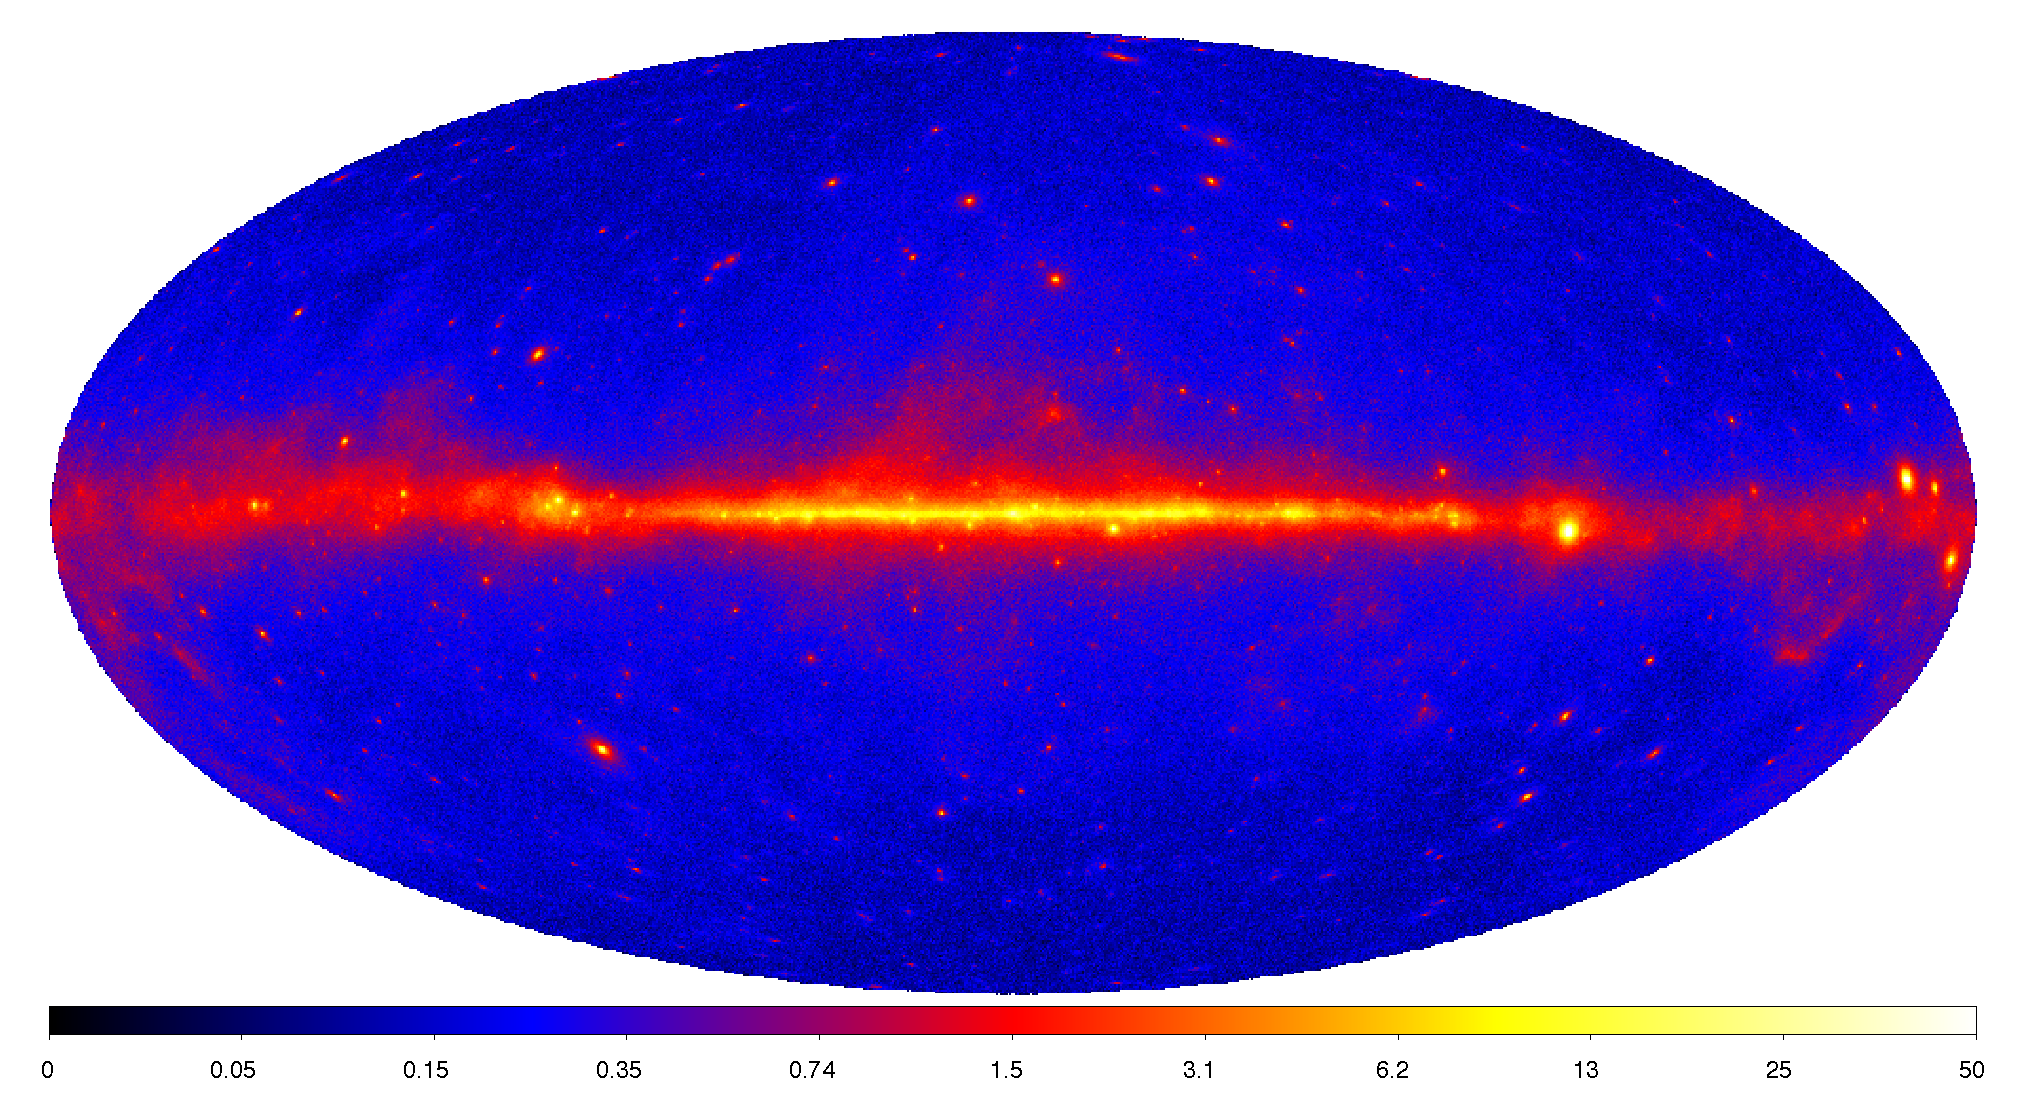
\includegraphics[width=\textwidth]{chapters/introduction/figures/lat_skymap_2fgl.pdf}
  \caption{...
  An Aitoff projection skymap of $\gamma$-ray sky observed by the
  \ac{LAT} in the energy range from $100\unitspace\mev$ to $10\unitspace\gev$
  in units of $10^{-7}\erg\cm^{-2}\second^{-1}\steradian^{-1}$.
  This figure is from \cite{nolan_2012_fermi-large}.
  }
  \figlabel{lat_skymap_2fgl}
\end{figure}

\begin{itemize}
  \item A variety of sources detected by \ac{LAT}:
\end{itemize}

\subsection{The Galactic Diffuse and Isotropic Gamma-ray Background}
\subseclabel{galactic_diffuse_and_isotropic}

\todo[inline]{Include discussion of modeling, if time permitting}

\begin{itemize}
  \item Discuss the historical Observations of galactic diffuse emission

    Mention how \gls{OSO-3} first detected the $gamma$-rays from the galaxy: \secref{history_gamma_ray_detectors}.

  \item GALPROP model of diffuse emission.
  Reference: \url{http://arxiv.org/abs/1202.4039}
  \item Emperical Ring model of galactic diffuse emisson.
  \item The isotropic background: \url{http://arxiv.org/abs/1002.3603}
\end{itemize}

\begin{itemize}
  \item Galactic diffuse emission is primarily composed of \ldots
  \item Something about how great galprop is.
  \item Something about
\end{itemize}


\subsection{\Actitle{2FGL}}

\Gls{2FGL} was a catalog by the \ac{LAT} collaboration containing XXX Sources.
\todo[inline]{Describe Catalog}

\begin{itemize}
  \item Citation is \cite{nolan_2012_fermi-large}
  \item Source classification method
  \item Number of sources detected by the \gls{LAT}
  \item Forward reference \chapref{maximum_likelihood_analysis},
    which does a more thorough description of likelihood analysis method.
  \item Source classes/associations
\end{itemize}

\subsection{\Actitle{2PC}}

\Gls{2PC} is a \ldots
\seclabel{second_pulsar_catalog}

\begin{itemize}
  \item Process of detecting Pulsars with the \gls{LAT}
  \item Number of pulsars detected by the \gls{LAT}
\end{itemize}

\subsection{\Acptitle{PWN} Detected by \Actitle{LAT}}

\subsubsection{Crab}

\subsubsection{Vela X}

\subsubsection{MSH 15-52}

\todo[inline]{Dig up HESS reference of HESS J1514-59.}

\subsubsection{\hessj{1825}}

\hessj{1825} is a cool source

HESS Detection: 
HESS Energy dependent morphology: \cite{aharonian_2006a_energy-dependent}

LAT Detection: \cite{grondin_2011_detection-pulsar}



\subsubsection{\hessj{1640}}

\hessj{1640} is also cool.

HESS detection:  \cite{aharonian_2006a_h.e.s.s.-survey}
Fermi detection: \cite{slane_2010_fermi-detection}

\subsubsection{\hessj{1857}}

\hessj{1857} is another good source.

LAT detection: \cite{rousseau_2012_fermi-lat-constraints}

\begin{enumerate}
  \item \url{http://arxiv.org/pdf/1206.3324v1.pdf}
\end{enumerate}

\subsubsection{J1023}

\ldots
